This test problem simulates an absorber obstruction in a vacuum.
An incoming flux beam at an angle of $45^\circ$ to the x-axis, travels
through a vacuum and collides with an absorber region. This test
problem shows how the beam diffuses transversely to the travel direction
and how the flux interacts at the upper left and lower right corners
of the absorber block.
Table \ref{tab:obstruction} summarizes the problem parameters.

%-------------------------------------------------------------------------------
\begin{table}[htb]\caption{Obstruction Test Problem Summary}
\label{tab:obstruction}
\centering
\begin{tabular}{l l}\toprule
\emph{Parameter} & \emph{Value}\\\midrule
Domain & $\mathcal{D} = (0,1)^2$\\
Initial Conditions & $u_0(\x)=0$\\
Boundary Conditions & $u(\x,t)=\left\{\begin{array}{c c c}
  1 & y = 0 & t > 0\\
  1 & x = 0 & t > 0
  \end{array}\right.$\\
Direction & $\di = \pr{\frac{1}{\sqrt{2}},\frac{1}{\sqrt{2}}}$\\
Cross Section & $\sigma(\x)=\left\{\begin{array}{c c}
    10 & \x \in (\frac{1}{3},\frac{2}{3})^2\\
    0  & \mbox{otherwise}
  \end{array}\right.$\\
Source & $q(\x,t)=0$\\
Speed & $\speed=1$\\
\bottomrule\end{tabular}
\end{table}
%-------------------------------------------------------------------------------

This test problem was run with a number of time discretizations, including
explicit (forward) Euler (FE), implicit (backward) Euler (BE), and steady-state (SS).
Run parameters are summarized in Table \ref{tab:obstruction_run}.

%-------------------------------------------------------------------------------
\begin{table}[htb]\caption{Obstruction Test Problem Run Parameters}
\label{tab:obstruction_run}
\centering
\begin{tabular}{l l}\toprule
\emph{Parameter} & \emph{Value}\\\midrule
Number of Cells & FE: $N_{cell} = 4096$\\
                & BE: $N_{cell} = 1024$\\
                & SS: $N_{cell} = 1024$\\
Time Discretization & Explicit Euler, Implicit Euler, Steady-State\\
End Time & $t = 2$ (or to steady-state)\\
CFL Number & FE: $\nu = 0.1$\\
           & BE: $\nu = 1.0$\\
Boundary Conditions & Strong Dirichlet with
  $\limiterletter_i^-=\limiterletter_i^+=1$\\
\midrule
Entropy Function & $\entropy(\scalarsolution) = \frac{1}{2}\scalarsolution^2$\\
Entropy Residual Coefficient & $\entropyresidualcoef = 0.1$\\
Entropy Jump Coefficient & $\entropyjumpcoef = 0.1$\\\midrule
FCT Solution Bounds & DMP\\
FCT Initial Guess & $\scalarsolution^{(0)} = \scalarsolution^{L}$\\
\bottomrule\end{tabular}
\end{table}
%-------------------------------------------------------------------------------

Figure \ref{fig:obstruction_fe} shows the explicit Euler results for the
low-order scheme and the EV-FCT scheme. The low-order solution
is relatively diffusive, and one can observe that the beam broadens as it
travels farther away from the absorber region. In the EV-FCT solution, this
broadening is not observable in the image, and the thickness of this
diffusive band is smaller. However, one can still observe some slight
``stair-stepping'' behavior, where the solution does not necessarily
lack monotonicity but some artificial plateaus have appeared.
Figure \ref{fig:obstruction_fe_visc} compares the low-order and entropy
viscosity profiles for this problem, using explicit Euler. The low-order
viscosity is shown on a linear scale, and the entropy viscosity is shown
on a log scale. The entropy viscosity is very large around the incident
edges of the absorber region, particularly the corners, and also
large along the edges of the unattenuated beam.

%-------------------------------------------------------------------------------
\begin{figure}[ht]
   \centering
   \begin{subfigure}{0.45\textwidth}
      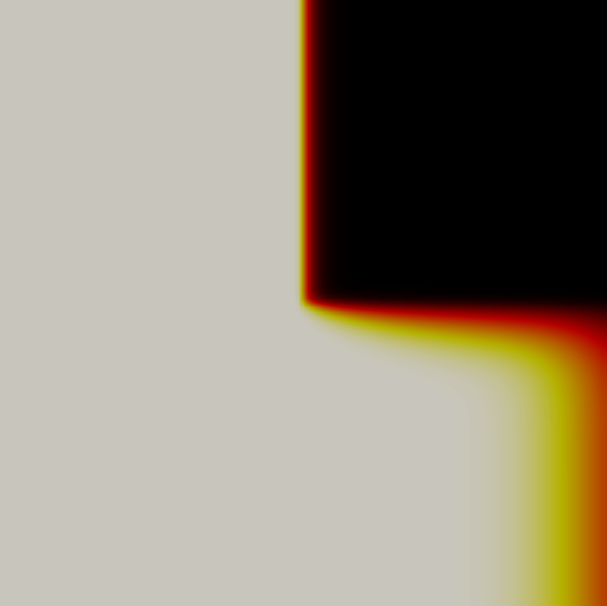
\includegraphics[width=\textwidth]
        {\contentdir/results/transport/obstruction/images/Low_FE.png}
      \caption{Low-order scheme}
   \end{subfigure}
   \begin{subfigure}{0.45\textwidth}
      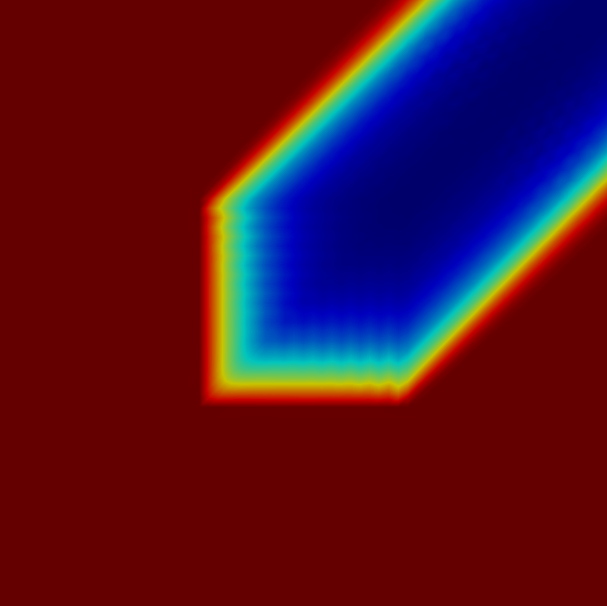
\includegraphics[width=\textwidth]
        {\contentdir/results/transport/obstruction/images/EVFCT_FE.png}
      \caption{EV-FCT scheme}
   \end{subfigure}
   \caption{Comparison of Solutions for the Obstruction Test
     Problem Using Explicit Euler Time Discretization with DMP Solution Bounds}
   \label{fig:obstruction_fe}
\end{figure}
%-------------------------------------------------------------------------------
%-------------------------------------------------------------------------------
\begin{figure}[ht]
   \centering
   \begin{subfigure}{0.45\textwidth}
      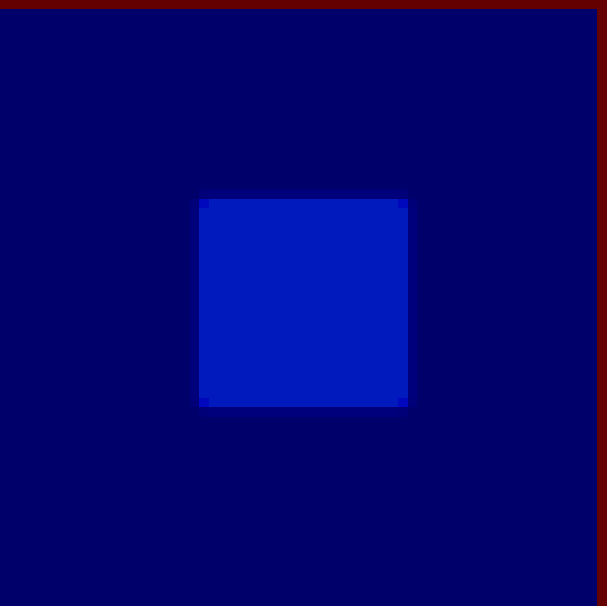
\includegraphics[width=\textwidth]
        {\contentdir/results/transport/obstruction/images/low_viscosity_FE_linearscale.png}
      \caption{Low-order Viscosity}
   \end{subfigure}
   \begin{subfigure}{0.45\textwidth}
      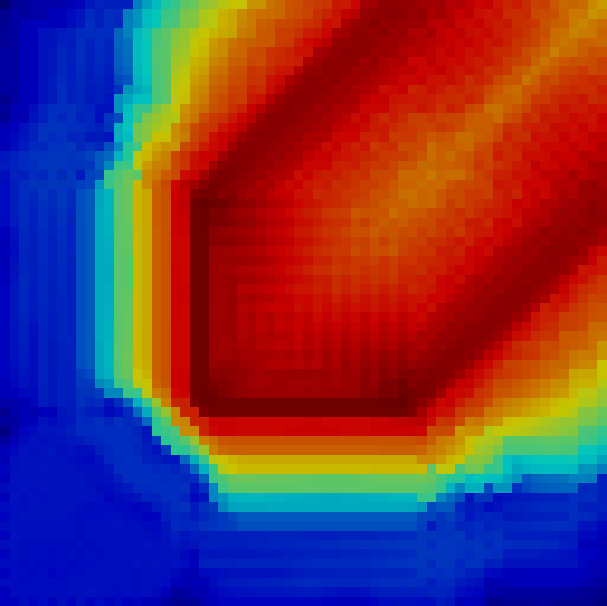
\includegraphics[width=\textwidth]
        {\contentdir/results/transport/obstruction/images/entropy_viscosity_FE_logscale.png}
      \caption{EV-FCT scheme}
   \end{subfigure}
   \caption{Comparison of Solutions for the Obstruction Test
     Problem Using Explicit Euler Time Discretization with DMP Solution Bounds}
   \label{fig:obstruction_fe_visc}
\end{figure}
%-------------------------------------------------------------------------------

Figure \ref{fig:obstruction_be} shows the EV-FCT results obtained using implicit Euler.
If comparing the EV-FCT solution to that obtained with explicit Euler, note
that the number of cells for the FE solution is 4 times the number of cells
used for BE and that the CFL for BE was 10 times as large as for FE. This is
why one can see the beam edges begin to drift outward for the implicit
Euler case - a steady-state was not reached with $t=2$ yet when the CFL $\nu=1$
is used, due to temporal diffusion.
Figure \ref{fig:obstruction_ss} shows the EV-FCT results obtained using
steady-state discretization.

%-------------------------------------------------------------------------------
\begin{figure}[ht]
   \centering
   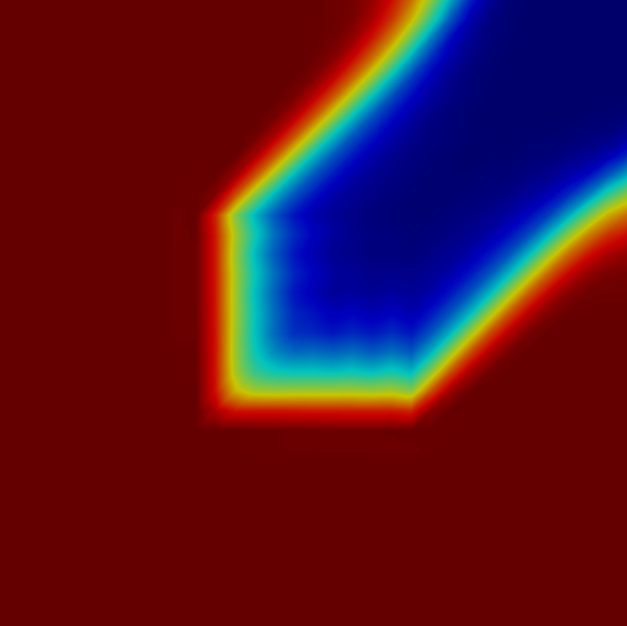
\includegraphics[width=\textwidth]
     {\contentdir/results/transport/obstruction/images/solution_BE.png}
   \caption{EV-FCT Solution for the Obstruction Test
     Problem Using Implicit Euler Time Discretization with DMP Solution Bounds}
   \label{fig:obstruction_be}
\end{figure}
%-------------------------------------------------------------------------------
%-------------------------------------------------------------------------------
\begin{figure}[ht]
   \centering
   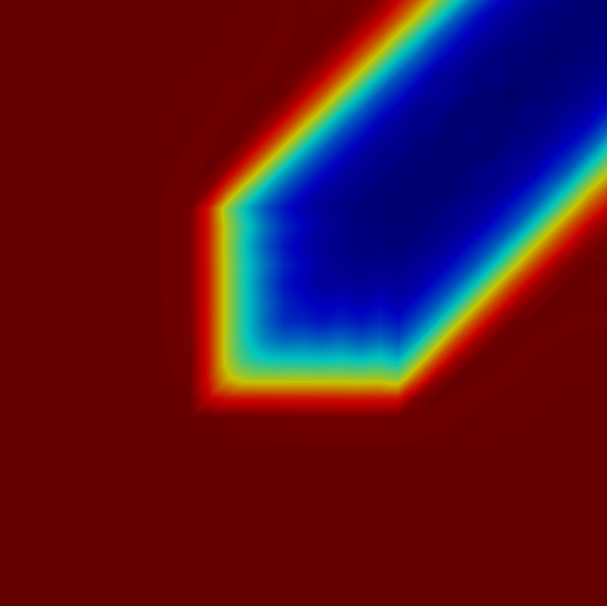
\includegraphics[width=\textwidth]
     {\contentdir/results/transport/obstruction/images/solution_SS.png}
   \caption{EV-FCT Solution for the Obstruction Test
     Problem Using Steady-State Time Discretization with DMP Solution Bounds}
   \label{fig:obstruction_ss}
\end{figure}
%-------------------------------------------------------------------------------

The fixed-point iteration schemes described in Sections
\ref{sec:nonlinear_iteration} and \ref{sec:fct_nonlinear_iteration} 
are used to converge the nonlinearities in the implicit and steady-state
entropy viscosity (EV) and FCT schemes.
The nonlinear solution of EV and FCT solutions is
shown to have significant convergence issues. These convergence
issues have most strongly been linked to the dimensionality of
the problem, mesh size, and CFL number.
The convergence criteria used in the nonlinear solver for the
nonlinear system $\mathbf{B}(\solutionvector)\solutionvector=\mathbf{s}$
(shown for each nonlinear scheme in Section \ref{sec:nonlinear_iteration}) is
\begin{equation}
  e^{(\ell)} = \|\mathbf{B}^{(\ell)}\solutionvector^{(\ell)}
    - \mathbf{s}^{(\ell)}\|_{\ell^2} < \epsilon=10^{-10}\eqc
\end{equation}
where $\|\mathbf{a}\|_{\ell^2}$ denotes the discrete L-2 norm of $\mathbf{a}$.

Table \ref{tab:obstruction_be_iterations_cfl} shows a study
of the number of nonlinear iterations required for
BE with 256 cells for a range of CFL numbers. In computing the EV-FCT
solution for a time step, one first computes the EV solution iteratively
and then computes the FCT solution iteratively; these two solves
in the EV-FCT solution are represented by the \emph{EV} and \emph{FCT} columns.
The sub-columns \emph{Total} and \emph{Avg.} correspond to the total
number of iterations in the transient and the average number of iterations
per time step, respectively. Entries of -- denote that convergence failed
during the transient for either EV or FCT, and the entry
``\textcolor{red}{\textbf{FAIL}}'' denotes which of the nonlinear
iterations (EV or FCT) caused the failure.
The results in the table
indicate that both EV and FCT iterations increase with increasing CFL
number but that the increase is more drastic with FCT. At a CFL of 20.0,
the FCT scheme fails to converge. As a general rule, the solution bounds
are larger with larger time steps, and there is more opportunity for
antidiffusive flux limiting coefficients to vary.

%-------------------------------------------------------------------------------
\begin{table}[htb]\caption{Nonlinear Iterations vs. CFL Number for the
  Obstruction Test Problem Using Implicit Euler Time Discretization with 256 Cells}
\label{tab:obstruction_be_iterations_cfl}
\centering
\begin{tabular}{c c c c c}\toprule
\emph{CFL} & \multicolumn{2}{c}{\emph{EV}} & \multicolumn{2}{c}{\emph{FCT}}\\
           & \emph{Total} & \emph{Avg.}    &  \emph{Total} & \emph{Avg.}\\\midrule
0.1  & 3999 &  8.14 & 3585 &   7.30\\
0.5  &  896 &  9.05 & 1499 &  15.14\\
1.0  &  501 & 10.02 &  970 &  19.40\\
5.0  &  157 & 15.70 & 1130 & 113.00\\
10.0 &   79 & 15.80 &  753 & 150.60\\
20.0 &   -- &    -- & \multicolumn{2}{c}{\textcolor{red}{\textbf{FAIL}}}\\
\bottomrule\end{tabular}
\end{table}
%-------------------------------------------------------------------------------

Table \ref{tab:obstruction_be_iterations_mesh} shows a study for backward
Euler (BE) time discretization with a
constant CFL of $\nu=1$, but a varying mesh size. This shows that the average
number of iterations per time step decreases with increasing mesh refinement,
although this effect is not drastic.

%-------------------------------------------------------------------------------
\begin{table}[htb]\caption{Nonlinear Iterations vs. Number of Cells for the
  Obstruction Test Problem Using Implicit Euler Time Discretization with CFL = 1}
\label{tab:obstruction_be_iterations_mesh}
\centering
\begin{tabular}{c c c c c}\toprule
$N_{cell}$ & \multicolumn{2}{c}{\emph{EV}} & \multicolumn{2}{c}{\emph{FCT}}\\
           & \emph{Total} & \emph{Avg.} &  \emph{Total} & \emph{Avg.}\\\midrule
64         & 261 & 10.44 &  699 & 27.96\\
256        & 501 & 10.02 & 1053 & 21.06\\
1024       & 827 &  8.35 & 2040 & 20.61\\
\bottomrule\end{tabular}
\end{table}
%-------------------------------------------------------------------------------

Table \ref{tab:obstruction_ss_iterations_mesh} shows a study for steady-state
where the mesh size is varied. These results show a different trend indicated
by Table \ref{tab:obstruction_be_iterations_mesh}.
For EV, the number of iterations required \emph{increases} with mesh refinement.
For FCT, the number of iterations required shows little or no relationship to
the mesh size. For very fine mesh refinements, the EV solution does not even
converge.

%-------------------------------------------------------------------------------
\begin{table}[htb]\caption{Nonlinear Iterations vs. Number of Cells for the
  Steady-State Obstruction Test Problem}
\label{tab:obstruction_ss_iterations_mesh}
\centering
\begin{tabular}{c c c}\toprule
$N_{cell}$ & \emph{EV} & \emph{FCT}\\\midrule
64         & 32 & 9284\\
256        & 59 & 440\\
1024       & 1072 & 3148\\
4096       & --   & --\\
\bottomrule\end{tabular}
\end{table}
%-------------------------------------------------------------------------------

\clearpage

